% \clearpage
% \newcommand{\dummyfigure}[3]{%
%     \begin{tikzpicture}
%         \draw [
%             thick, 
%             pattern=north east lines, 
%             pattern color=black!10, 
%             inner sep=0,
%         ] 
%         (0,0) rectangle (#1 - \pgflinewidth, #2 - \pgflinewidth) 
%         node[
%             pos=0.5, 
%             align=center, 
%             font=\small, 
%             text width=#1,
%         ] {
%             #3 \\[2mm] 
%         };
%     \end{tikzpicture}%
% }


\begin{figure}[t]
  \centering
  \makebox[\textwidth][c]{%
    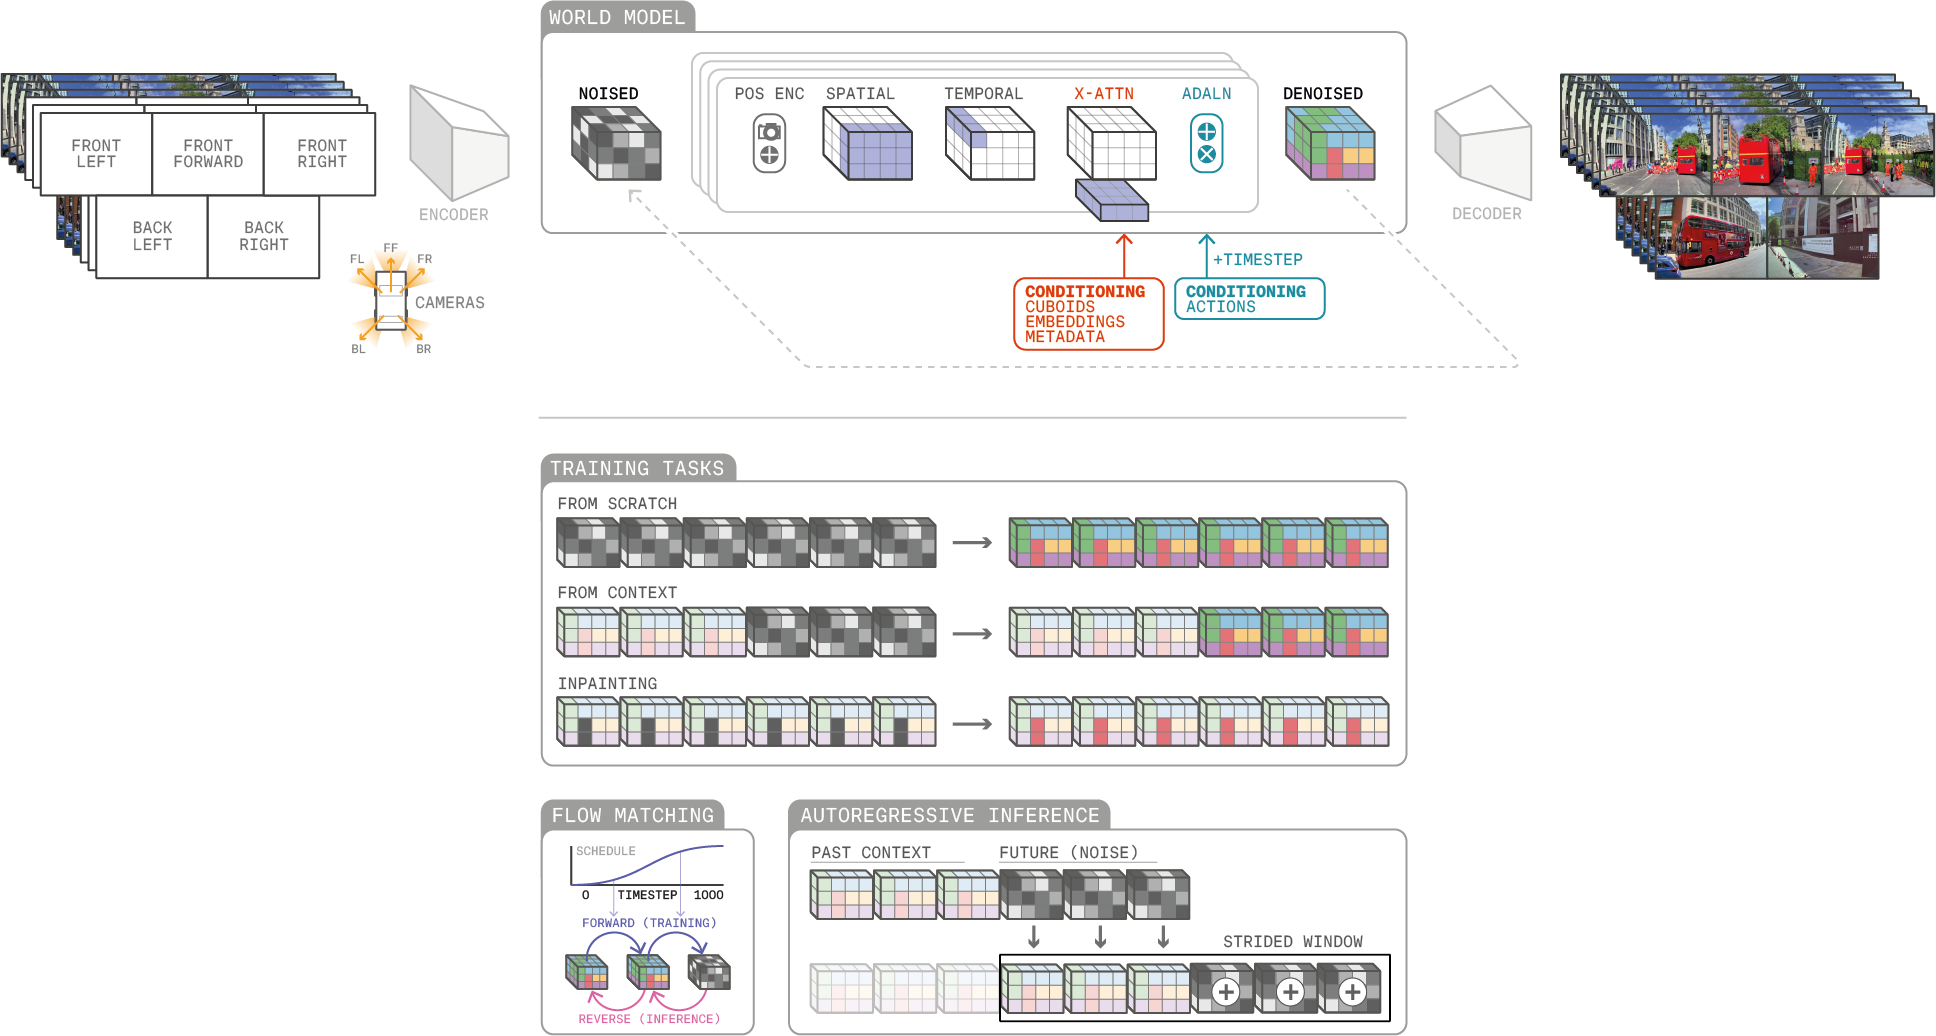
\includegraphics[width=1\textwidth]{Figures/wm_diagram.png}%
  }
  \caption{\textbf{GAIA-2 world model}. The architecture schematic shows full surround camera views independently encoded by a video tokenizer. The combined multi-camera latents are used as past context and linearly interpolated with sampled noise. We add camera parameters along with positional encodings before passing the latents through a space-time factorized transformer. Conditioning is implemented via cross-attention and adaptive layer norm. The latents are denoised into future latents, conditioned on various inputs, including actions, 3D bounding boxes, metadata, and scenario embeddings. The denoised latents are then decoded back to pixel space by the video tokenizer. Below, we depict the various tasks GAIA-2 is trained on, including from scratch generations, 
  context rollouts, and spatial inpainting. At inference, we can generate beyond the window duration GAIA-2 was trained on by taking overlapping strides to generate new frames conditioned on previously generated frames.}
  \label{fig:wm-arch}
  \vspace{-10pt}
\end{figure}



\section{Model}
\label{section:model}
%High level description of GAIA-2
% Autonomous driving simulation requires generative models that are both high-fidelity and controllable across multiple modalities. 
GAIA-2 is a surround-view video generative world model with structured conditioning, multi-camera coherence, and high spatial-temporal resolution. The architecture (\Cref{fig:wm-arch}) is composed of two primary components: a video tokenizer and a latent world model. Together, these modules enable GAIA-2 to generate realistic and semantically coherent video across multiple viewpoints with rich conditional control.

The video tokenizer compresses the raw high-resolution video into a compact, continuous latent space, preserving semantic and temporal structure. This compact representation enables efficient learning and generation at scale. The world model then learns to predict future latent states, conditioned on past latent states, actions, and a diverse set of domain-specific control signals. It can also be used to generate novel states completely from scratch and modify video content through inpainting. The predicted latent states are subsequently decoded back into pixel space using the video tokenizer decoder.

In contrast to most latent diffusion models, GAIA-2 employs a much higher spatial compression rate (e.g., $32\times$ vs. the more typical $8\times$), which is offset by increasing the channel dimension of the latent space (e.g., 64 channels instead of 16). This yields fewer but semantically richer latent tokens. The resulting advantages are twofold: (1) shorter latent sequences enable faster inference and better memory efficiency, and (2) the model demonstrates improved ability to capture video content and temporal dynamics. This parameterization strategy is inspired by prior work on compact latent representations~\cite{dcae,ltx}.

%Brief textual comparison with GAIA-1
Unlike its predecessor GAIA-1~\cite{gaia1-2023}, which relied on discrete latent variables, GAIA-2 employs a continuous latent space, improving temporal smoothness and reconstruction fidelity. Furthermore, GAIA-2 introduces a flexible conditioning interface that supports ego-vehicle actions, dynamic agent states (e.g., 3D bounding boxes), structured metadata, CLIP and scenario embeddings, and camera geometry. This design enables robust control over scene semantics and agent behavior during generation, while ensuring cross-view consistency and temporal coherence.


\subsection{Video Tokenizer}

The video tokenizer compresses pixel-space video into a compact latent space that is continuous and semantically structured. It is composed of a space-time factorized transformer with an asymmetric encoder-decoder architecture (with 85M and 200M parameters, respectively). The encoder extracts spatiotemporally downsampled latents that are temporally independent; the decoder reconstructs full-frame video from these latents using temporal context for temporal consistency. 

\begin{figure}[t]
  \centering
  \makebox[\textwidth][c]{%
    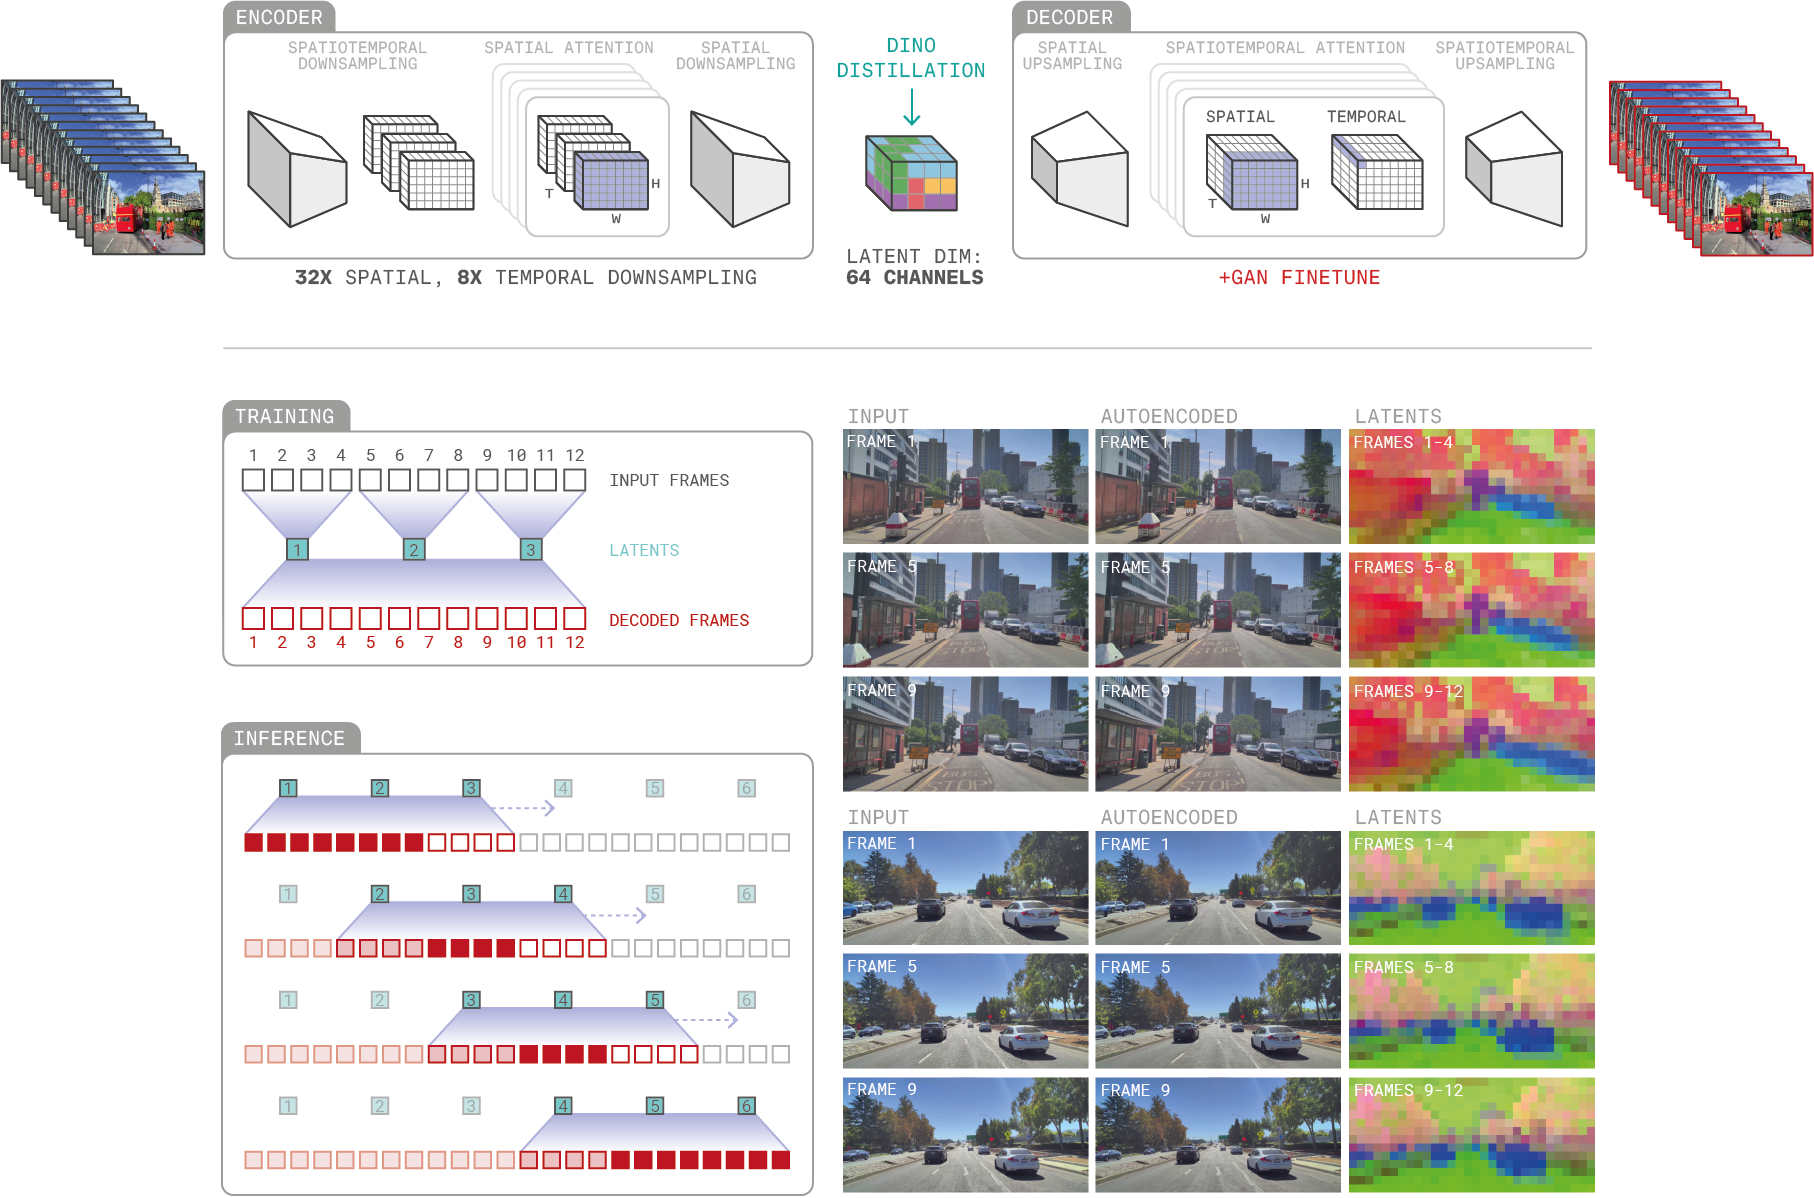
\includegraphics[width=1\textwidth]{Figures/video_tokenizer_diagram.png}%
  }
  \caption{\textbf{GAIA-2 video tokenizer}. The architecture schematic depicts input frames spatiotemporally downsampled into temporally independent latents. A high spatial compression rate is compensated for by an increased latent channel dimension. Latents are decoded back to video frames, leveraging full spatiotemporal attention to ensure temporal consistency. To autoencode long sequences, we employ a rolling inference mechanism where current latents are decoded using past and future context in a sliding window fashion. The examples show input frames, decoded frames, and a visualization of the latent space. The first 3 principal components of the latent features are mapped to RGB values. Notably, the latent space is semantically stable across frames and across samples.}
    \label{fig:video-tokenizer}
\end{figure}


\subsubsection{Encoder}
Given an input video $(\rvi_1, ..., \rvi_{T_v})$, the encoder $e_{\phi}$ computes latent tokens $(\rvz_1, ..., \rvz_{T_L}) = e_{\phi}(\rvi_1, ..., \rvi_{T_v})$, where $T_v$ corresponds to the number of video frames and $T_L$ the number of latents. Let us denote by $H_v \times W_v$ the spatial resolution of the video frames and $H\times W$ the spatial resolution of the latent tokens. The encoder downsamples spatially by a factor $\frac{H_v}{H} = 32$ and temporally by a factor $\frac{T_v}{T_L} = 8$. The latent dimension is $L=64$, which results in a total compression of ($\frac{T_v \times H_v \times W_v \times 3}{T_L \times H \times W \times L} =384)$ with $(T_v, H_v, W_v) = (24, 448, 960)$ and $(T_L, H, W) = (3, 14, 30)$.

This downsampling is achieved by temporally striding the input frames by $2\times$ and the following modules:
\begin{enumerate}
    \item A downsampling convolutional block with stride $2 \times 8 \times 8$ (time, height, width) followed by another downsampling convolutional block with stride $2 \times 2 \times 2$ (both operating at embedding dimension $512$).
    \item A series of $24$ spatial transformer blocks with dimension $512$ and $16$ heads.
    \item A final convolution with stride $1 \times 2 \times 2$, followed by a linear projection to $2L$ channels to model a Gaussian distribution over latents. Note that the latent dimension is doubled as the encoder predicts the mean and standard deviation of a Gaussian distribution. During both training and inference, the latents are sampled from this resulting distribution.
\end{enumerate}

\subsubsection{Decoder}
The decoder architecture is:
\begin{enumerate}
    \item A linear projection from the latent dimension to the embedding dimension followed by a first upsampling convolutional block with stride $1 \times 2 \times 2$ (upsampling is achieved with a depth-to-space module \citep{shi16}).
    \item A series of 16 space-time factorized transformer blocks with dimension $512$ and $16$ heads.
    \item An upsampling convolutional block with stride $2 \times 2 \times 2$ followed by $8$ space-time factorized transformer blocks with dimension $512$ and $16$ heads.
    \item A final upsampling convolutional block with stride $2 \times 8 \times 8$ and dimension $3$ corresponding to the pixel RGB channels.
\end{enumerate}

A key difference between the encoder and decoder is that the encoder independently maps $8$ consecutive video frames to a single temporal latent, while the decoder jointly decodes the $T_L=3$ temporal latents to $T_v=24$ video frames for temporal consistency. During inference, the video frames are decoded with a sliding window. The logic is shown in diagrams `\textit{Training}' and `\textit{Inference}' of \Cref{fig:video-tokenizer}.

\subsubsection{Training Losses}
The video tokenizer is trained with a combination of pixel reconstruction and latent space losses:
\begin{itemize}
    \item Image reconstruction with $L_1$, $L_2$, and perceptual losses \citep{Johnson2016Perceptual}.
    \item DINO \citep{oquab2023dinov2} distillation on the latent features through a cosine similarity loss, encouraging semantic alignment with pre-trained representations. The video frames are encoded with the DINO model and temporally downsampled with linear interpolation to match the dimensionality of the latent features.
    \item Kullback-Leibler divergence loss \citep{kingma14} with respect to a standard Gaussian distribution to regularize the latent space. 
\end{itemize}

To improve visual quality, we further fine-tune the decoder with a GAN loss \citep{esser21} using a 3D convolutional discriminator and the image reconstruction losses, while keeping the encoder frozen. The discriminator is a series of residual 3D convolutional blocks with base channel 64, stride 2 in time and space with 3D blur pooling \citep{zhang2019shiftinvar}, channel multipliers [2, 4, 8, 8], 3D instance normalization, and LeakyReLU with slope $0.2$. It uses spectral normalization \citep{miyato18} and the original GAN loss implemented with a softplus activation function.



\subsection{World Model}
% Continuous latent space with rectified flow matching
The latent world model predicts future latent states conditioned on past latents, actions, and a rich set of conditioning inputs. It is implemented as a space-time factorized transformer with 8.4B parameters and is trained using flow matching~\cite{lipman23} for stability and sample efficiency.

Let $\rvx_{1:T} \in \mathbb{R}^{T \times N \times H \times W \times L}$ be the input latents, where $T$ is the temporal window and $N$ is the number of cameras. The input latents are obtained by independently encoding each camera view with the encoder $e_{\phi}$. At each timestep $t$, we also provide an action vector $\rva_t$ and a conditioning vector $\rvc_t$.


\subsubsection{Architecture}

The world model is a space-time factorized transformer with hidden dimension $C$. Each action $\rva_t$ is embedded to $\R^C$, and the conditioning vector $\rvc_t$ embedded to $\R^{K\times C}$, where $K$ corresponds to the number of conditioning variables. The flow matching time $\tau \in [0, 1]$ is also mapped to $\R^C$ using a sinusoidal encoding \cite{ho2020}.

Flow matching time $\tau$ and action $\rva_t$ are injected into each transformer block through the adaptive layer norm \cite{peebles2023scalable}, while we use cross-attention for the other conditioning variables $\rvc_t$. We have found that action conditioning was more accurate when using adaptive layer norm over cross-attention. As the action affects every spatial token, the adaptive layer norm provides an explicit information gateway instead of having to rely on a learnable attention mechanism.

Regarding positional encoding, we independently encode: (i) spatial token position with a sinusoidal embedding, (ii) camera timestamp with a sinusoidal embedding followed by a small MLP, and (iii) camera geometry (distortion, intrinsic, and extrinsics) with learnable linear layers. All these positional encodings are added to the input latents at the beginning of each transformer block, similar to \cite{polyak2024movie}. 

The world model contains $22$ space-time factorized transformer blocks with hidden dimension $C=4096$ and $32$ heads. Each transformer block contains a spatial attention (over space and cameras), a temporal attention, a cross-attention, and an MLP layer with an adaptive layer norm. For increased training stability, we use query-key normalization \cite{dehghani2023scaling} before each attention layer.


\subsubsection{Losses}
At training time, we randomly sample the number of context frames $t \in \{0, ..., T-1\}$ where $t=0$ corresponds to from scratch generation. We also sample a flow matching time $\tau \in [0, 1]$ according to a pre-defined distribution (see \Cref{subsubsection:flow-matching-distribution} for more details). The context latents $\rvx_{1:t} $ are unchanged, while the future latents $\rvx_{t+1:T} $ are linearly interpolated with random Gaussian noise $\rvepsilon_{t+1:T} \sim \mathcal{N}(\vzero, \mI)$. 
% 
\begin{equation}
    \rvx_{t+1:T}^{\tau} = \tau \rvx_{t+1:T} + (1 - \tau) \rvepsilon_{t+1:T}
\end{equation}

The velocity target vector $\rvv_{t+1:T}$ is the difference between target latents and random noise:
% 
\begin{equation}
    \rvv_{t+1:T} = \rvx_{t+1:T} - \rvepsilon_{t+1:T}
\end{equation}

The world model $f_{\theta}$ predicts the target velocity $\rvv_{t+1:T}$ conditioned on context latents $\rvx_{1:t}$, actions $\rva_{1:T}$ and conditioning variables $\rvc_{1:T}$.
% 
\begin{equation}
    \hat{\rvv}_{t+1:T} = f_{\theta}(\rvx_{t+1:T}^{\tau} | \rvx_{1:t}, \rva_{1:T}, \rvc_{1:T}, \tau)
\end{equation}

The model is trained with an $L_2$ loss between the predicted and the target velocity.
% 
\begin{equation}
    \mathcal{L}_{\text{world-model}} = \mathbb{E}_{t \sim P(t), \tau \sim p(\tau)} [||\rvv_{t+1:T} - \hat{\rvv}_{t+1:T} ||^2]
\end{equation}
% 
where $t \sim P(t)$ denotes the distribution of context frames and $\tau \sim p(\tau)$ the distribution of flow matching time.

\subsubsection{Conditioning}
\label{subsubsection:conditioning}
GAIA-2 supports rich and structured conditioning inputs that enable fine-grained control over the generated scenes. These inputs include ego-vehicle actions, dynamic agent properties, scene-level metadata, camera configurations, timestamp embedding, and external latent representations such as CLIP or proprietary scenario embeddings. The conditioning mechanisms are integrated into the world model through a combination of adaptive layer normalization (for action), additive modules (for camera geometry and timestamp), and cross-attention (for all other variables).

\paragraph{Camera Parameters.} We compute separate embeddings for intrinsics, extrinsics, and distortion, which are then summed to form a unified camera encoding. For intrinsics, we extract focal lengths and principal point coordinates from the intrinsic matrix, normalize them, and project them into a shared latent space. Extrinsics and distortion coefficients are similarly processed through their respective encoders to yield compact representations. This configuration allows the model to effectively incorporate real-world camera variations. \Cref{fig:camera-rigs} illustrates the top three most common camera rig configurations in the training dataset.


\paragraph{Video Frequency.} To account for variable video frame rates, GAIA-2 uses timestamp conditioning. Each timestamp is: (\textit{i}) Normalized relative to the present time and scaled to the range $[-1, 1]$, (\textit{ii}) Transformed using sinusoidal functions (Fourier feature encoding), and (\textit{iii}) Passed through an MLP to produce a vector in the shared latent space. This encoding captures both low- and high-frequency temporal variation and enables the model to reason effectively over videos recorded at different rates.

\paragraph{Action.} The ego-vehicle action is parameterized by speed and curvature. Since these quantities span multiple orders of magnitude, we use a symmetric logarithmic transformation \textit{symlog} \cite{webber12} for normalization:
% 
\begin{equation}
    \text{symlog}(y) = \text{sign}(y)
    \frac{\log(1 + s|y|)}{\log(1 + s|y_{\text{max}}|)}
\end{equation}
% 
Here, $y$ represents speed or curvature, and $s$ is a scale factor:
For curvature (units: $m^{-1}$, range: $0.0001$ to $0.1$), we use $s = 1000$ to amplify low values. For speed (units: m/s, range: $0$ to $75$), we use $s = 3.6$ to express values in km/h.
The result is a compact representation scaled to $[-1, 1]$, improving training stability.

\paragraph{Dynamic Agents.}
To represent surrounding agents, we use 3D bounding boxes predicted by a 3D object detector~\cite{wang2023streampetr} re-trained on our dataset. Each box encodes the 3D location, orientation, dimensions, and category of an agent. The 3D boxes are projected into the 2D image plane and normalized, yielding $f_i \in \mathbb{R}^{T \times N \times B \times 13}$ conditioning features where $T$ denotes the number of temporal latents, $N$ the number of cameras, and $B$ the maximum number of 3D bounding boxes (zero-padding as needed). Each feature dimension is embedded independently and aggregated via a single-layer MLP.

To enhance model robustness and generalizability, we implement dropout at both the feature dimension and instance levels during training. Specifically, feature dimensions are dropped out with a probability of $p = 0.3$, allowing the model to operate under incomplete information at inference. This setup allows, for example, conditioning on 2D projected boxes without specifying the 3D locations of instances, or omitting orientations to let the model predict the most plausible orientation based on other conditions.

 At the instance level, for each camera, we sample a frame $t \in \{1, ..., T\}$ and calculate the number of detected instances $N_{\text{instances}}$. We then sample the number of instances to condition on $n\in \{0, ..., \min(B, N_{\text{instances}})\}$, and apply dropout to the instances exceeding this sample size. This allows the model to adapt to a variable number of dynamic agents during inference. Note that while keeping $n$ constant across time, we do not use instance tracking, allowing the model to independently determine whether the conditioning features across frames belong to the same or different instances.


\paragraph{Metadata.} Metadata features are categorical and embedded using dedicated learnable embedding layers. These include: Country, weather, time of day; Speed limits; Number and types of lanes (e.g., bus, cycle); Pedestrian crossings, traffic lights and their states; One-way road indicators and intersection types.
These embeddings allow GAIA-2 to learn nuanced relationships between scene-level features and their effects on behavior, enabling simulation of both typical and rare scenarios.


\paragraph{CLIP Embedding.} To enable semantic scene conditioning, GAIA-2 supports conditioning on CLIP embeddings~\cite{radford21}. During training, we extract CLIP features using the image encoder on video frames. At inference, these can be replaced with CLIP text encoder outputs from natural language prompts. All CLIP embeddings are projected into the model’s latent space using a learnable linear projection.
This enables zero-shot control over scene semantics through natural language or visual similarity.


\paragraph{Scenario Embedding.} GAIA-2 can also be conditioned on scenario embeddings obtained from an internal proprietary model trained to encode driving-specific information. These embeddings compactly capture ego-action and scene context, such as road layout and agent configurations. The scenario vectors are projected via a learnable linear layer into the latent space before integration into the transformer.
This allows high-level scenario generation from a compact abstract representation.


\subsubsection{Flow matching Time Distribution}
\label{subsubsection:flow-matching-distribution}
A critical factor for training the world model under the flow matching framework is the distribution of the flow matching time $\tau$. This distribution determines how frequently the model sees latent inputs that are close to real latents versus heavily perturbed.

We use a bimodal logit-normal distribution with two modes:
\begin{itemize}
    \item A primary mode centered at $\mu = 0.5$, $\sigma = 1.4$, sampled with probability $p = 0.8$. This biases the model towards learning with low-to-moderate noise levels. Empirically, this encourages learning useful gradients, as even small amounts of noise can significantly perturb high-capacity latents.
    \item A secondary mode centered at $\mu = -3.0$, $\sigma = 1.0$, sampled with probability $p = 0.2$. This concentrates training on nearly pure noise regions around $\tau = 0$, helping the model learn spatial structures and low-level dynamics, such as ego-motion or object trajectories.
\end{itemize}
This bimodal strategy ensures that training is effective across both low and high-noise regimes, improving generalization and sample quality.

In addition, the input latents $\rvx_t$ are normalized by their mean $\mu_x$ and standard deviation $\sigma_x$, following~\cite{rombach2022highresolution}, to ensure their magnitude matches that of the added Gaussian noise. This avoids scale mismatch between the signal and the perturbation, which can otherwise degrade training dynamics.